% !Mode:: "TeX:UTF-8"
% !TEX program = xelatex
% 使用 XeLaTeX 编译；Overleaf 请在 Menu -> Compiler 中选择 XeLaTeX。
\def\usewhat{xelatex}
\documentclass[twoside,openany,UTF8,fontset=none]{ctexbook}

% 引入信息中枢
% !Mode:: "TeX:UTF-8"

% ============================================================
% 0. 打印模式配置
% ============================================================
% true  = 保留空白页 (标准双面打印，章首页强制在奇数页)
% false = 删除空白页 (连续排版，章首页可出现在偶数页)
\newcommand{\isOpenBlankPage}{false}
% ============================================================
% 1. 报告题目
% ============================================================
\newcommand{\myTitle}{大语言模型空间建模能力的认知边界与逻辑一致性挖掘分析}
\newcommand{\myETitle}{Mining Cognitive Boundaries and Logical Consistency of Large Language Models in Spatial Reasoning}

% ============================================================
% 2. 分类与密级
% ============================================================
\newcommand{\myClassification}{TP18} % 中图分类号
%\newcommand{\myUDC}{004}              % UDC号，暂不需要
\newcommand{\mySecurityLevel}{公开}    % 密级（公开/秘密/机密/绝密）
\newcommand{\myStudentId}{23070215}   % 学号

% ============================================================
% 3. 作者与课程信息
% ============================================================
\newcommand{\myAuthor}{张驰}
\newcommand{\myCollege}{信息学部}
\newcommand{\myCourseName}{数据挖掘}
\newcommand{\myTopicDirection}{大语言模型；空间推理；数据挖掘}
\newcommand{\myInstructor}{（请填写指导教师）}
\newcommand{\myInstructorTitle}{（请填写职称）}

% ============================================================
% 4. 报告基本信息
% ============================================================
\newcommand{\myReportType}{本科课程报告}
\newcommand{\mySource}{数据挖掘课程项目}
\newcommand{\mySubmitDate}{2026年5月}
\newcommand{\myConferringUnit}{北京工业大学}

% ============================================================
% 5. 时间
% ============================================================
\newcommand{\myYear}{\the\year}
\newcommand{\myMonth}{\CJKnumber{\the\month}}


% 引入版式设置
% !Mode:: "TeX:UTF-8"
% 北京工业大学数据挖掘课程报告宏包配置
\usepackage{iftex}
\ifPDFTeX
  \PackageError{BJUTCourseReport}
    {This template must be compiled with XeLaTeX or LuaLaTeX}
    {In Overleaf, open Menu -> Compiler and choose XeLaTeX.}
\fi
% ============================================================
% 1. 页面布局与尺寸 (核心：适配双面打印与36行网格)
% ============================================================
\usepackage[
    a4paper,
    top=25mm,
    bottom=25mm,
    inner=27mm,    % 装订内侧边距
    outer=27mm,    % 外侧边距
    headheight=5mm,
    headsep=7.5mm, % 页眉位置
    footskip=12mm, % 页脚位置
    lines=36,      % 显式指定行数 (配合 format.tex 中的字号设置)
    heightrounded, % 自动微调高度以容纳整数行
]{geometry}

% ============================================================
% 2. 数学公式支持
% ============================================================
\usepackage{amsmath}   % 基础数学宏包
\usepackage{amssymb}   % 数学符号
\usepackage{amsfonts}  % 数学字体
\usepackage{bm}        % 数学粗体
\usepackage[amsmath,thmmarks,hyperref]{ntheorem} % 定理环境

% ============================================================
% 3. 图表支持
% ============================================================
\usepackage{graphicx}  % 插图核心宏包
\graphicspath{{figures/}} % 图片默认路径

\usepackage{booktabs}  % 三线表 (\toprule, \midrule, \bottomrule)
\usepackage{multirow}  % 表格多行合并
\usepackage{longtable} % 跨页长表格
\usepackage{array}     % 增强表格功能
\usepackage{caption}   % 图表标题定制 (替代老旧的 ccaption)
\usepackage[below]{placeins} % 防止浮动体跨过 \FloatBarrier
\usepackage{bicaption} % 支持双语图注
% ============================================================
% 4. 格式控制与辅助工具
% ============================================================
\usepackage{titlesec}  % 章节标题格式控制
\usepackage{titletoc}  % 目录格式控制
\usepackage{fancyhdr}  % 页眉页脚控制
\usepackage{enumitem}  % 列表环境控制
\usepackage{setspace}  % 行距控制
\usepackage{xcolor}    % 颜色支持
\usepackage{fontspec}  % 字体高级支持 (配合 XeLaTeX)
\usepackage{calc}      % 长度计算

% ============================================================
% 5. 参考文献
% ============================================================
\usepackage[sort&compress,numbers,super]{natbib} % 引用优化 (排序+压缩: [1-3])

% ============================================================
% 6. 代码高亮
% ============================================================
\usepackage{listings}

% 定义颜色
\definecolor{codegreen}{rgb}{0,0.6,0}
\definecolor{codegray}{rgb}{0.5,0.5,0.5}
\definecolor{codepurple}{rgb}{0.58,0,0.82}
\definecolor{backcolour}{rgb}{0.95,0.95,0.92} % 护眼淡灰色背景

% 设置代码样式
\lstdefinestyle{mystyle}{
    backgroundcolor=\color{backcolour},
    commentstyle=\color{codegreen}\itshape, % 注释斜体+绿色
    keywordstyle=\color{blue}\bfseries,     % 关键字蓝色+加粗
    numberstyle=\tiny\color{codegray},      % 行号样式
    stringstyle=\color{codepurple},         % 字符串样式
    basicstyle=\zihao{5}\ttfamily,          % 字号五号 + 等宽字体
    breakatwhitespace=false,
    breaklines=true,                 % 自动换行
    captionpos=b,                    % 标题在底部
    keepspaces=true,
    numbers=left,                    % 行号在左侧
    numbersep=5pt,
    showspaces=false,
    showstringspaces=false,
    showtabs=false,
    tabsize=4,
    frame=shadowbox,                 % 阴影边框 (也可以选 single)
    rulesepcolor=\color{red!20!green!20!blue!20}, % 阴影颜色
    xleftmargin=2em,                 % 左侧缩进，防止行号溢出
    xrightmargin=1em,                % 右侧缩进
    framexleftmargin=1.5em           % 边框左侧扩充
}

\lstset{style=mystyle}

% ============================================================
% 6.5. 伪代码算法环境
% ============================================================
\usepackage[ruled,vlined,linesnumbered]{algorithm2e}

% ============================================================
% 8. 字体设置：适配 Overleaf / TeX Live
% ============================================================
\usepackage{fontspec}

\ifPDFTeX\else
  \setmainfont{TeX Gyre Termes}
  \setsansfont{TeX Gyre Heros}
  \setmonofont{TeX Gyre Cursor}

  \newcommand{\BJUTSetCJKFamilies}[3]{%
    \setCJKmainfont{#1}%
    \setCJKsansfont{#2}%
    \setCJKmonofont{#2}%
    \setCJKfamilyfont{zhsong}{#1}%
    \setCJKfamilyfont{zhhei}{#2}%
    \setCJKfamilyfont{zhkai}{#3}%
    \providecommand{\songti}{}%
    \providecommand{\heiti}{}%
    \providecommand{\kaishu}{}%
    \providecommand{\fangsong}{}%
    \renewcommand{\songti}{\CJKfamily{zhsong}}%
    \renewcommand{\heiti}{\CJKfamily{zhhei}}%
    \renewcommand{\kaishu}{\CJKfamily{zhkai}}%
    \renewcommand{\fangsong}{\CJKfamily{zhsong}}%
  }

  \IfFontExistsTF{Noto Serif CJK SC}{%
    \BJUTSetCJKFamilies{Noto Serif CJK SC}{Noto Sans CJK SC}{Noto Serif CJK SC}%
    \IfFontExistsTF{Noto Sans Mono CJK SC}{\setCJKmonofont{Noto Sans Mono CJK SC}}{}%
  }{%
    \IfFontExistsTF{FandolSong-Regular}{%
      \BJUTSetCJKFamilies{FandolSong-Regular}{FandolHei-Regular}{FandolKai-Regular}%
      \setCJKmonofont{FandolFang-Regular}%
    }{%
      \BJUTSetCJKFamilies{AR PL UMing CN}{AR PL UMing CN}{AR PL UMing CN}%
    }%
  }%
\fi

% ============================================================
% 7. 超链接设置
% ============================================================
\usepackage[
    unicode=true,
    bookmarksnumbered=true,
    bookmarksopen=true,
    colorlinks=false, % 打印版通常要求黑色链接
    pdfborder={0 0 0}, % 去掉链接红框
    pdfkeywords={},
    pdfstartview=FitH
]{hyperref}

% ============================================================
% 生僻字显示方案：字体已在上方设置，通常无需额外处理。
\endinput

% !Mode:: "TeX:UTF-8"
% 北京工业大学数据挖掘课程报告格式定义

\makeatletter

% ============================================================
% 0. 兼容性定义
% ============================================================
\newcommand{\erhao}{\zihao{2}}
\newcommand{\xiaoer}{\zihao{-2}}
\newcommand{\sanhao}{\zihao{3}}
\newcommand{\xiaosan}{\zihao{-3}}
\newcommand{\sihao}{\zihao{4}}
\newcommand{\xiaosi}{\zihao{-4}}
\newcommand{\wuhao}{\zihao{5}}
\newcommand{\xiaowu}{\zihao{-5}}
\newcommand{\song}{\songti}
\newcommand{\hei}{\heiti}
\newcommand{\kai}{\kaishu}
\newcommand{\fs}{\fangsong}

% ============================================================
% 1. 基础行网格 (正文 36 行)
% ============================================================
\renewcommand\normalsize{
  % 重置行距倍数为 1.0，防止倍数叠加
  \renewcommand{\baselinestretch}{1.0}

  % 计算逻辑：版心 247mm / 36行 ≈ 19.45pt (微调值，防止溢出)
  \@setfontsize\normalsize{12pt}{19.45pt}

  % 强制取消段落间距
  \setlength{\parskip}{0pt}

  % 调整公式间距
  \setlength\abovedisplayskip{6pt plus 2pt minus 2pt}
  \setlength\belowdisplayskip{6pt plus 2pt minus 2pt}
  \setlength\abovedisplayshortskip{0pt plus 2pt}
  \setlength\belowdisplayshortskip{4pt plus 2pt minus 2pt}
  \let\@listi\@listI
}
\def\defaultfont{\normalsize\selectfont}
\setlength{\parindent}{2em}
\punctstyle{hangmobanjiao}
\setlist{nosep}

% ============================================================
% 2. 章节标题格式
% ============================================================
% 设置编号深度为 3 (显示 1.1.1.1)
\setcounter{secnumdepth}{3}

% 一级标题 (Chapter)
% 保持原样，或者段后也可以稍微改小
\titleformat{\chapter}{\centering\zihao{-3}\heiti}{\thechapter}{1em}{}
\titlespacing{\chapter}{0pt}{6pt}{6pt}

% 二级标题 (Section) - 1.1
% 将段后间距设为 0pt，防止标题高度超标导致跳行
\titleformat{\section}{\zihao{4}\heiti}{\thesection}{1em}{}
\titlespacing{\section}{0pt}{6pt}{0pt}

% 三级标题 (Subsection) - 1.1.1
% 为保持视觉一致，段后间距设为 0pt，段前间距设为 6pt
\titleformat{\subsection}{\zihao{4}\heiti}{\thesubsection}{1em}{}
\titlespacing{\subsection}{0pt}{6pt}{0pt}

% 四级标题 (Subsubsection) - 1.1.1.1
\titleformat{\subsubsection}{\zihao{-4}\heiti}{\thesubsubsection}{1em}{}
%\titlespacing{\subsubsection}{0pt}{0pt}{0pt}
\titleformat{\subsubsection}{\zihao{-4}\heiti}{\thesubsubsection}{1em}{}
\titlespacing{\subsubsection}{0pt}{6pt}{0pt}

% ============================================================
% 3. 页眉页脚 (奇偶页不同)
% ============================================================
\usepackage{fancyhdr}

% --- 1. 定义一个通用的页眉页脚配置命令 (供后面调用) ---
\newcommand{\bjutHeaderConfig}{
    \fancyhf{} % 清空
    \fancyhead[CO]{\songti\zihao{-5} 北京工业大学数据挖掘课程报告}
    \fancyhead[CE]{\songti\zihao{-5} \leftmark}
    \fancyfoot[C]{\rmfamily\zihao{-5} \thepage}
    \renewcommand{\headrulewidth}{0.5pt}
}

% --- 2. 设置默认的 fancy 样式 (用于正文非首页) ---
\pagestyle{fancy}
\bjutHeaderConfig  % <--- 关键：让普通页加载配置！

% --- 3. 设置默认的 plain 样式 (用于章首页) ---
% 默认情况下，我们在 format 里让 plain 和 fancy 长得一样
% 这样正文里的章首页就会有页眉
\fancypagestyle{plain}{
    \bjutHeaderConfig
}

% 章节标记格式
\renewcommand{\chaptermark}[1]{\markboth{\thechapter\quad #1}{}}
% ============================================================
% 4. 目录样式
% ============================================================
\renewcommand{\contentsname}{\zihao{3}\heiti 目\quad 录}
\setcounter{tocdepth}{2}

\newcommand{\worddots}{\titlerule*[3pt]{.}}

% --- 章 (一级标题) ---
% 格式：顶格 (无缩进要求)
\titlecontents{chapter}[0pt]
              {\vspace{0pt}\normalsize\songti\bfseries}
              {\rmfamily\thecontentslabel\hspace{0.5em}}
              {}
              {\hspace{0.5em}\worddots\contentspage}

% --- 节 (二级标题) ---
% 要求：之前有 1 个中文字符的空格 -> [1\ccwd]
\titlecontents{section}[1\ccwd]
              {\vspace{0pt}\normalsize\songti}
              {\rmfamily\thecontentslabel\hspace{0.5em}}
              {}
              {\hspace{0.5em}\worddots\contentspage}

% --- 小节 (三级标题) ---
% 要求：之前有 2 个中文字符的空格 -> [2\ccwd]
\titlecontents{subsection}[2\ccwd]
              {\vspace{0pt}\normalsize\songti}
              {\rmfamily\thecontentslabel\hspace{0.5em}}
              {}
              {\hspace{0.5em}\worddots\contentspage}
% ============================================================
% 5. 参考文献环境
% ============================================================
\renewenvironment{thebibliography}[1]{
    % 标题带编号
    \chapter{\bibname}

    % 直接使用正文默认设置，不强制单倍行距
    % 这样行距就会自动继承 \normalsize 的 19.52pt

    \list{\@biblabel{\@arabic\c@enumiv}}
         {\settowidth\labelwidth{\@biblabel{#1}}
          \leftmargin\labelwidth
          \advance\leftmargin\labelsep
          % 如果列表项之间太松散，可以保留下面这行；如果想完全和正文段落一致，就注释掉
          %\setlength{\itemsep}{0pt}
          \setlength{\itemsep}{0pt}   % 条目与条目之间的额外间距
          \setlength{\parsep}{0pt}    % 条目内段落之间的间距 (这个最关键！)
          \setlength{\parskip}{0pt}   % 段落前后的间距
          \setlength{\topsep}{0pt}    % 列表与上方正文的间距
          \setlength{\partopsep}{0pt} % 列表与上方页面的间距
          \usecounter{enumiv}
          \let\p@enumiv\@empty
          \renewcommand\theenumiv{\@arabic\c@enumiv}}
    \sloppy
    \clubpenalty4000
    \@clubpenalty \clubpenalty
    \widowpenalty4000
    \sfcode`\.\@m}
   {\def\@noitemerr
     {\@latex@warning{Empty `thebibliography' environment}}
    \endlist}
% ============================================================
% 6. 其他配置
% ============================================================
\renewcommand{\tablename}{表}
\renewcommand{\figurename}{图}
\renewcommand{\thefigure}{\thechapter-\arabic{figure}}
\renewcommand{\thetable}{\thechapter-\arabic{table}}
\renewcommand{\theequation}{\thechapter-\arabic{equation}}

\DeclareCaptionFont{captionwuhao}{\zihao{5}}
\DeclareCaptionFont{captionhei}{\heiti}
\captionsetup{font=captionwuhao, labelsep=quad}
\captionsetup[figure]{name=图, labelfont=captionhei, textfont=captionhei}
\captionsetup[table]{name=表, labelfont=captionhei, textfont=captionhei}

\def\temp{\relax}
\let\temp\addcontentsline
\gdef\addcontentsline{\phantomsection\temp}

% 项目成果列表
% \newlist{publist}{enumerate}{1}
% \setlist[publist]{label={[\arabic*]}, leftmargin=3em, itemsep=0pt, parsep=0pt, topsep=0pt}
\newlist{publist}{enumerate}{1}
\setlist[publist]{
    label={[\arabic*]},
    leftmargin=3em,
    itemsep=0pt,  % 条目间距
    parsep=0pt,   % 段落间距
    topsep=0pt,   % 与上方文本的间距
    partopsep=0pt,
    % 让列表内部行距跟随正文
    % 如果觉得太紧，可以试试 \setstretch{1.3} 之类的
    % 但既然要求“单倍行距”，这里默认跟随当前环境即可
}


% \def\cleardoublepage{\clearpage\if@twoside \ifodd\c@page\else
%   \hbox{}
%   \thispagestyle{empty}
%   \newpage
%   \if@twocolumn\hbox{}\newpage\fi\fi\fi}

% ============================================================
% 7. 覆盖 ctex 的默认编号设置
% ============================================================
\ctexset{
    chapter = {
        number = \arabic{chapter},
        name = {}, % 去掉“第”和“章”
    },
    section = {
        number = \thechapter.\arabic{section},
        name = {},
    },
    subsection = {
        % 关键修复：原本这里可能有 name={（,）}，我们要把它清空
        number = \thesection.\arabic{subsection},
        name = {},
        format = \zihao{4}\heiti, % 确保字体也是黑体
    },
    subsubsection = {
        number = \thesubsection.\arabic{subsubsection},
        name = {},
        format = \zihao{-4}\heiti,
    }
}
% ============================================================
% 8. 图表与公式格式 (修正双语图注前缀)
% ============================================================
\renewcommand{\tablename}{表}
\renewcommand{\figurename}{图}
\renewcommand{\thefigure}{\thechapter-\arabic{figure}}
\renewcommand{\thetable}{\thechapter-\arabic{table}}
\renewcommand{\theequation}{\thechapter-\arabic{equation}}

% 注册字体
\DeclareCaptionFont{captionwuhao}{\zihao{5}}
\DeclareCaptionFont{captionhei}{\heiti}
\DeclareCaptionFont{captioneng}{\rmfamily} % 英文用衬线体

% 基础设置
\captionsetup{
    font=captionwuhao,
    labelsep=quad, % 序号后空一格
    singlelinecheck=true % 单行居中
}

% --- 双语图注核心配置 ---
% lang=1 (中文) 配置
\captionsetup[figure][bi-first]{
    name=图,
    labelfont=captionhei,
    textfont=captionhei
}
% lang=2 (英文) 配置：关键是这里！
\captionsetup[figure][bi-second]{
    name=Fig.,           % 前缀改为 Fig.
    labelfont=captioneng,
    textfont=captioneng
}

% 表格同理
\captionsetup[table][bi-first]{
    name=表,
    labelfont=captionhei,
    textfont=captionhei
}
\captionsetup[table][bi-second]{
    name=Table,          % 前缀改为 Table
    labelfont=captioneng,
    textfont=captioneng
}

% ============================================================
% 9. 代码与算法的中文化重命名
% ============================================================
\renewcommand{\lstlistingname}{代码} % 将 Listing 改为 代码
\renewcommand{\algorithmcfname}{算法} % 将 Algorithm 改为 算法

% 修正 listings 的编号格式为 "章-序号" (如 代码 3-1)
\AtBeginDocument{
  \renewcommand{\thelstlisting}{\thechapter-\arabic{lstlisting}}
}

% ============================================================
% 10. 智能空白页控制 (由 metadata.tex 中的开关控制)
% ============================================================
\usepackage{ifthen} % 需要引入逻辑判断宏包

\makeatletter
\def\cleardoublepage{
  \clearpage
  % 如果是双面打印模式
  \if@twoside
    % 检查开关是否为 true
    \ifthenelse{\equal{\isOpenBlankPage}{true}}{
      % --- 模式 A：保留空白页 (标准做法) ---
      \ifodd\c@page
        % 当前是奇数页时，插入空白页，保证新章节从奇数页开始。
        \else
        % 当前是偶数页，不做操作，新章节直接从奇数页开始。
      \fi
      % 实际上 LaTeX 默认的 \cleardoublepage 就够了，
      % 但为了处理页眉页脚，我们通常会重写它：
      \ifodd\c@page\else
        \hbox{}
        \thispagestyle{empty} % 空白页不显页码
        \newpage
        \if@twocolumn\hbox{}\newpage\fi
      \fi
    }{
      % --- 模式 B：强制删除空白页 (紧凑做法) ---
      % 直接什么都不做，等于 \clearpage
      % 这样新章节就会紧接着上一章结束的页面开始
    }
  \fi
}

\bibpunct{[}{]}{,}{s}{}{;}

\makeatother


\begin{document}

% ============================================================
% 1. 绝对无页码区 (封面、声明、摘要)
% ============================================================

% 封面、声明与摘要页不显示页眉页脚
\fancypagestyle{plain}{
    \fancyhf{}
    \renewcommand{\headrulewidth}{0pt}
}
\pagestyle{empty}

% 临时禁用空白页
\let\oldcleardoublepage\cleardoublepage
\renewcommand{\cleardoublepage}{\clearpage}

% !Mode:: "TeX:UTF-8"
% 封面：北京工业大学数据挖掘课程报告

\begin{titlepage}
    \thispagestyle{empty}

    \vspace*{2.2cm}

    \begin{center}
        {\zihao{1}\song\bfseries 北京工业大学 \par}
        \vspace{0.8cm}
        {\xiaoer\song\bfseries 数据挖掘课程报告 \par}
    \end{center}

    % 报告题目
    \vspace{2.2cm}
    \begin{center}
        \renewcommand{\baselinestretch}{1.5}\selectfont
        {\xiaoer\song\bfseries \myTitle \par}
        %\vspace{1cm}
        {\xiaosan\bfseries\rmfamily \myETitle \par}
    \end{center}

    \vfill

    % 个人信息栏
    {
        \sanhao\hei
        \renewcommand\arraystretch{1.8}

        \par
        \noindent
        % 右侧信息栏与模板封面标题保持视觉平衡
        \makebox[4.5cm]{}\begin{minipage}{12cm}
            \begin{tabular}{r @{\hspace{2pt}} c @{\hspace{4pt}} l}
                \makebox[5.6em][s]{学院名称} & ： & \makebox[8cm][l]{\myCollege} \\
                \makebox[5.6em][s]{课程名称} & ： & \makebox[8cm][l]{\myCourseName} \\
                \makebox[5.6em][s]{学生姓名} & ： & \makebox[8cm][l]{\myAuthor} \\
                \makebox[5.6em][s]{指导教师} & ： & \makebox[8cm][l]{\myInstructor \quad \myInstructorTitle} \\
            \end{tabular}
        \end{minipage}
    }

    \vspace{3cm}

    % 日期
    \begin{center}
        \sanhao\hei
        \mySubmitDate
    \end{center}

    \vspace{2cm}
    \clearpage
\end{titlepage}

% !Mode:: "TeX:UTF-8"
% 扉页：北京工业大学数据挖掘课程报告

\begin{titlepage}
    \thispagestyle{empty}

    % 顶部信息栏
    \noindent
    \song\xiaosi
    分类号：\makebox[3cm][l]{\myClassification} \hfill 学校代码：10005 \\[10pt]
    密级：\makebox[3cm][l]{\mySecurityLevel} \hfill 学号：\myStudentId

    % 报告题目
    \vspace{4.5cm}
    \begin{center}
        \renewcommand{\baselinestretch}{1.5}\selectfont
        {\xiaoer\song\bfseries \myTitle \par}
        %\vspace{0.8cm}
        {\xiaosan\bfseries\rmfamily \myETitle \par}
    \end{center}

    % 3. 详细信息栏
    \vspace{4.5cm}
    \begin{center}
        \xiaosi\song
        \renewcommand\arraystretch{1.6}

        \begin{tabular}{r @{\hspace{4pt}} c @{\hspace{4pt}} l}
            \makebox[7em][s]{课程名称} & ： & \myCourseName \\
            \makebox[7em][s]{研究方向} & ： & \myTopicDirection \\
            \makebox[7em][s]{指导教师姓名} & ： & \myInstructor \quad \myInstructorTitle \\
            \makebox[7em][s]{学生姓名} & ： & \myAuthor \\
            \makebox[7em][s]{报告类型} & ： & \myReportType \\
            \makebox[7em][s]{提交日期} & ： & \mySubmitDate \\
            \makebox[7em][s]{课题来源} & ： & \mySource \\
            \makebox[7em][s]{所在学校} & ： & \myConferringUnit \\
        \end{tabular}
    \end{center}

    \clearpage
\end{titlepage}

% !Mode:: "TeX:UTF-8"

\setlength{\baselineskip}{23pt}
\selectfont

\begin{center}
    {\sanhao\song\bfseries 北\hspace{0.5em}京\hspace{0.5em}工\hspace{0.5em}业\hspace{0.5em}大\hspace{0.5em}学 \par}
    \vspace{0.5em}
    {\xiaosi\song\bfseries 课程报告原创性声明 \par}
\end{center}

\par
\indent 本人郑重声明：所呈交的课程报告，是本人在课程学习和教师指导下，独立进行实验设计、数据采集、特征抽取和数据挖掘分析所取得的成果。除文中特别加以标注引用的内容外，本报告不包含任何其他个人或集体已经发表或撰写过的作品成果。对本文研究和实现做出重要贡献的个人和集体，均已在文中以明确方式标明。本人完全知晓本声明的法律结果由本人承担。

\par \vspace{1em}
\noindent \hspace*{2em} 作者签名：
\par
\noindent \hspace*{2em} 日期：\hspace{2em} 年 \hspace{1em} 月 \hspace{1em} 日

\par \vspace{3em}

\begin{center}
    {\xiaosi\song\bfseries 课程报告使用授权声明 \par}
\end{center}

\par
\indent 本人完全了解学校有关保留、使用课程报告的规定，同意学校保留并向有关部门或机构送交课程报告的复印件和电子版，允许课程报告被查阅和借阅。学校可以将本课程报告的全部或部分内容编入有关数据库进行检索，可以采用影印、缩印或扫描等复制手段保存和汇编课程报告。

\par \vspace{1em}
\noindent
\makebox[20em][l]{作者签名：} 日期：\hspace{2em} 年 \hspace{1em} 月 \hspace{1em} 日
\par
\noindent
\makebox[20em][l]{指导教师签名：} 日期：\hspace{2em} 年 \hspace{1em} 月 \hspace{1em} 日

\vfill
\defaultfont
\clearpage

% !Mode:: "TeX:UTF-8"

\chapter*{\centering \sanhao\song\bfseries 摘\quad 要}

\xiaosi\song
\setstretch{1.5}

本文围绕“电动轮椅能否在狭窄楼梯转角处完成 90 度转弯”这一空间推理任务，构建多层级 Prompt 数据集，将大语言模型的回答视为可挖掘的行为数据，分析模型在自然语言描述、参数化描述和数学建模描述之间的判断稳定性与认知边界。实验设计包含 20 个空间场景、3 个描述层级和 5 类无关干扰条件，形成 300 条基础 Prompt；随后采集模型回复，并抽取最终判断、推理步骤、公式使用、坐标系使用和错误类型等行为特征。

在数据挖掘阶段，本文设计了准确率统计、层级一致性、噪声翻转率、决策树、K-Means 聚类和 FP-Growth 关联规则等分析方法，用于识别模型在空间建模任务中的典型失效模式。该框架能够回答三个核心问题：第一，形式化几何描述是否一定提升模型判断准确率；第二，材质颜色、环境噪声、光照和情绪压力等无关信息是否会诱发模型判断翻转；第三，不同模型在空间推理任务中呈现出怎样的行为边界和错误模式。

当前报告基于项目已有代码和数据产物搭建完整分析框架，后续可在真实模型多轮采集完成后补充具体统计数值、典型错误样例和最终结论。该项目展示了如何将大语言模型回复转化为结构化行为数据，并使用数据挖掘方法分析模型能力边界。

\vspace{0.8cm}

\noindent {\hei\xiaosi 关键词：} 大语言模型；空间推理；数据挖掘；Prompt 工程；关联规则

% !Mode:: "TeX:UTF-8"

\chapter*{\centering \sanhao\bfseries ABSTRACT}

\xiaosi
\setstretch{1.5}

This report studies the cognitive boundaries of large language models in a controlled spatial reasoning task. Taking the wheelchair turning problem in a narrow stair corner as the fixed scenario, the project constructs prompts with different description levels and irrelevant perturbations, collects model responses, and extracts behavioral features such as final judgment, reasoning steps, formula usage, coordinate-system usage, and error category.

The analysis framework combines descriptive accuracy statistics, level consistency, noise-induced flip rate, decision tree analysis, K-Means clustering, and FP-Growth association rule mining. It aims to answer whether formal geometric descriptions improve model reliability, whether irrelevant environmental information changes model judgments, and what failure patterns appear in different models. This version provides a structured report framework based on the current project code and output artifacts. Final numerical findings can be added after multi-model response collection is completed.

\vspace{0.8cm}

\noindent {\bfseries\xiaosi Key words:} Large language model, Spatial reasoning, Data mining, Prompt engineering, Association rule mining


% ============================================================
% 2. 目录区 (恢复页码 I, II...)
% ============================================================

% 恢复双面打印逻辑 (如果需要)
\let\cleardoublepage\oldcleardoublepage
\cleardoublepage

\frontmatter          % 开启页码计数 (i, ii...)
\pagenumbering{Roman} % 强制大写罗马数字

% 目录区显示页脚页码
\fancypagestyle{plain}{
    \fancyhf{}
    \fancyfoot[C]{\rmfamily\zihao{-5} \thepage} % 目录页脚显示页码
    \renewcommand{\headrulewidth}{0pt}
}
\pagestyle{plain}

\tableofcontents

% ============================================================
% 3. 正文部分 (恢复正常)
% ============================================================
\mainmatter
\pagenumbering{arabic}

% 正文普通页：有页眉与页脚
\pagestyle{fancy}
\fancyhf{}
\fancyhead[CO]{\songti\zihao{-5} 北京工业大学数据挖掘课程报告}
\fancyhead[CE]{\songti\zihao{-5} \leftmark}
\fancyfoot[C]{\rmfamily\zihao{-5} \thepage}
\renewcommand{\headrulewidth}{0.5pt}

% 正文章首页：与普通页保持一致
\fancypagestyle{plain}{
    \fancyhf{}
    \fancyhead[CO]{\songti\zihao{-5} 北京工业大学数据挖掘课程报告}
    \fancyhead[CE]{\songti\zihao{-5} \leftmark}
    \fancyfoot[C]{\rmfamily\zihao{-5} \thepage}
    \renewcommand{\headrulewidth}{0.5pt}
}

\defaultfont

% !Mode:: "TeX:UTF-8"

\chapter{绪论}

\section{研究背景}

大语言模型在常识问答、代码生成和文本分析等任务中表现突出，但其是否真正具备稳定的空间建模能力仍需要通过可控实验验证。空间推理问题通常同时包含自然语言理解、几何约束识别、数量关系比较和逻辑一致性保持等要求，因此适合作为分析模型认知边界的实验载体。

本项目选择“电动轮椅在狭窄楼梯转角处能否顺利完成 90 度转弯”作为固定任务。该问题具有现实空间约束，同时又可以被改写为自然语言描述、参数化描述和形式化建模描述三种层级。与直接求解几何可通行性不同，本报告关注的是模型如何回答、为何出错，以及哪些描述变化会诱发回答翻转。

\section{研究目标}

本报告拟完成以下目标：

\begin{enumerate}
    \item 构建包含描述层级、干扰条件和场景临界性的 Prompt 实验矩阵；
    \item 自动化采集不同模型在同一空间任务上的回复；
    \item 从回复文本中抽取可量化行为特征；
    \item 使用数据挖掘方法识别模型的准确率差异、逻辑一致性、噪声敏感性和典型失效模式；
    \item 为课程报告和答辩提供可复现的数据、图表和结论框架。
\end{enumerate}

\section{项目技术路线}

项目整体流程如图 \ref{fig:pipeline} 所示：首先生成多层级 Prompt，然后调用 mock 或真实模型 API 采集回复；随后从回复中抽取最终判断、公式使用、坐标建模和错误类别等特征；最后进行统计分析、聚类分析和关联规则挖掘。

\begin{figure}[htbp]
    \centering
    \fbox{\parbox{0.86\textwidth}{
    Prompt 生成 $\rightarrow$ 模型回复采集 $\rightarrow$ 行为特征抽取 $\rightarrow$ 统计分析 / 聚类 / 关联规则 $\rightarrow$ 报告与可视化
    }}
    \bicaption{项目数据挖掘流程}{Data mining workflow of the project}
    \label{fig:pipeline}
\end{figure}

\section{本文组织结构}

第 2 章介绍数据集构造与实验变量设计；第 3 章说明模型回复采集和行为特征工程；第 4 章介绍准确率统计、聚类、决策树和 FP-Growth 等挖掘方法；第 5 章给出实验结果分析框架；最后总结当前工作并讨论后续完善方向。
      % 绪论
% !Mode:: "TeX:UTF-8"

\chapter{数据集构造与实验设计}

\section{空间场景生成}

实验以楼梯转角和电动轮椅几何参数为核心，生成多个空间场景。每个场景包含楼梯净宽、平台进深、轮椅宽度、轮椅长度、最小转弯半径等字段。项目中使用的参考余量定义为：

\begin{equation}
margin = \min(W - w,\ D - R)
\label{eq:margin}
\end{equation}

其中，$W$ 表示楼梯通道净宽，$w$ 表示轮椅宽度，$D$ 表示平台有效进深，$R$ 表示保守转弯半径。该参考余量不直接告诉模型，而是用于实验标注与后续评价。

\section{Prompt 描述层级}

实验将同一空间场景转写为三个描述层级，如表 \ref{tab:levels} 所示。该设计用于比较模型在自然语言直觉、参数比较和形式化几何建模三种语境下的行为差异。

\begin{table}[htbp]
    \centering
    \bicaption{Prompt 描述层级设计}{Design of prompt description levels}
    \begin{tabular}{lll}
        \toprule
        层级 & 描述方式 & 实验目的 \\
        \midrule
        L1 & 自然语言描述 & 测试模型是否依赖空间常识和直觉判断 \\
        L2 & 具体参数描述 & 测试模型能否正确使用尺寸和阈值信息 \\
        L3 & 数学建模描述 & 测试模型面对形式化几何约束时的稳定性 \\
        \bottomrule
    \end{tabular}
    \label{tab:levels}
\end{table}

\section{干扰条件设计}

为了检验模型是否会被无关环境信息带偏，实验为每个 Prompt 设置 5 类干扰条件。干扰项本身不改变空间几何约束，但可能影响模型的语义注意力分配。

\begin{table}[htbp]
    \centering
    \bicaption{无关干扰条件设计}{Design of irrelevant perturbation conditions}
    \begin{tabular}{ll}
        \toprule
        干扰标签 & 示例内容 \\
        \midrule
        none & 不添加无关信息 \\
        material\_color & 楼梯扶手颜色、墙面材质 \\
        ambient\_noise & 现场说话声和环境噪声 \\
        lighting & 光照偏暗、地面干燥等状态 \\
        emotional\_pressure & 使用者着急、旁观者催促 \\
        \bottomrule
    \end{tabular}
    \label{tab:noise}
\end{table}

\section{数据规模}

默认配置包含 20 个空间场景、3 个描述层级和 5 类干扰条件，因此单模型单轮采样形成：

\begin{equation}
20 \times 3 \times 5 = 300
\label{eq:prompt-size}
\end{equation}

条 Prompt。若比较 3 个模型并重复采样 3 次，则总回复量可达到 $300 \times 3 \times 3 = 2700$ 条。该规模能够支持准确率、翻转率、聚类和关联规则等多种数据挖掘分析。
      % 数据集构造与实验设计
% !Mode:: "TeX:UTF-8"

\chapter{数据采集与特征工程}

\section{采集流程}

项目通过 Python 脚本完成从 Prompt 生成到模型回复采集的流程。核心文件包括：

\begin{itemize}
    \item \texttt{scripts/01\_generate\_prompts.py}：生成 Prompt 矩阵；
    \item \texttt{scripts/02\_collect\_responses.py}：调用 mock 或真实模型 API；
    \item \texttt{scripts/03\_build\_features.py}：从回复文本中抽取行为特征；
    \item \texttt{scripts/04\_analyze.py}：执行统计分析、聚类和关联规则挖掘。
\end{itemize}

采集脚本支持断点续采，能够跳过已经存在的 $(model, repeat, prompt\_id)$ 组合，避免接口调用重复。真实模型采集时，应记录模型名称、采集时间、temperature、最大输出长度和失败重试情况，保证实验可追溯。

\section{数据文件说明}

项目中的主要数据文件如表 \ref{tab:data-files} 所示。

\begin{table}[htbp]
    \centering
    \bicaption{项目主要数据文件}{Main data files of the project}
    \begin{tabular}{ll}
        \toprule
        文件路径 & 内容说明 \\
        \midrule
        \texttt{data/prompts.csv} & Prompt 实验矩阵 \\
        \texttt{data/raw/model\_responses.csv} & 模型原始回复 \\
        \texttt{data/processed/behavior\_features.csv} & 行为特征表 \\
        \texttt{outputs/tables/*.csv} & 统计表、聚类结果和关联规则 \\
        \texttt{outputs/figures/*.png} & 热力图、雷达图和聚类图 \\
        \bottomrule
    \end{tabular}
    \label{tab:data-files}
\end{table}

\section{行为特征抽取}

模型原始回复通常是多段自然语言文本，无法直接进行统计分析。因此，需要将回复转换为结构化行为特征。本文关注的主要特征如表 \ref{tab:features} 所示。

\begin{table}[htbp]
    \centering
    \bicaption{模型回复行为特征}{Behavioral features extracted from model responses}
    \begin{tabular}{ll}
        \toprule
        字段 & 含义 \\
        \midrule
        ai\_judgment & 模型最终判断，包含能通过、不能通过、不确定 \\
        is\_correct & 模型判断是否与参考标签一致 \\
        reasoning\_steps & 回复中的推理步骤数量 \\
        has\_formula & 是否出现公式、比较符号或变量表达 \\
        uses\_coordinate & 是否使用坐标系、包络线等建模语言 \\
        error\_category & 错误回复对应的失效模式类别 \\
        \bottomrule
    \end{tabular}
    \label{tab:features}
\end{table}

\section{失效模式定义}

本项目将错误回复初步归纳为以下几类：概念混淆、计算崩溃、直觉过拟合、噪声牵引、单位混乱和信息不足。后续正式报告可结合典型样例，说明每类错误在文本中的具体表现。
      % 数据采集与特征工程
% !Mode:: "TeX:UTF-8"

\chapter{数据挖掘方法}

\section{描述性统计与准确率分析}

首先按模型、Prompt 层级、干扰条件和场景临界性统计准确率。该部分用于回答“哪个模型在哪类描述上更稳定”这一基础问题，并为后续可视化提供数据。

\section{层级一致性分析}

层级一致性用于衡量同一场景从 L1 到 L3 描述变化时，模型判断是否保持一致。如果模型在 L3 形式化描述中反而更容易出错，则说明形式化符号并不必然带来更强空间建模能力。

\section{噪声翻转率分析}

噪声翻转率衡量加入无关信息后，模型相对无噪声版本的最终判断是否发生变化。该指标可以识别模型是否过度关注颜色、噪声、光照和情绪压力等非几何因素。

\section{决策树与聚类分析}

决策树用于解释哪些特征最能区分正确与错误回复；K-Means 聚类用于根据准确率、一致性、公式使用率、坐标系使用率、噪声翻转率等指标划分模型行为类型。例如，某些模型可能表现为“符号逻辑型但计算链不稳定”，另一些模型可能表现为“自然语言直觉型但参数敏感性较低”。

\section{FP-Growth 关联规则挖掘}

FP-Growth 用于挖掘“条件组合 $\rightarrow$ 结果模式”的关联关系 \cite{han2000mining}。例如，可以分析如下规则：

\begin{equation}
\{level=L3,\ has\_noise=1\} \Rightarrow error\_category=calculation\_collapse
\label{eq:rule}
\end{equation}

这类规则有助于从大量回复中提炼可解释的失效路径，是本项目体现数据挖掘价值的重要部分。
      % 数据挖掘方法
% !Mode:: "TeX:UTF-8"

\chapter{实验结果与分析框架}

本章为后续完善报告时的结果承载框架。若真实模型采集已经完成，可直接从 \texttt{outputs/tables} 与 \texttt{outputs/figures} 中补充统计结果。

\section{整体准确率}

建议在此处插入 \texttt{outputs/tables/accuracy\_by\_level.csv} 的关键数值，并结合图 \ref{fig:accuracy} 说明不同模型在 L1、L2、L3 下的准确率差异。

\begin{figure}[htbp]
    \centering
    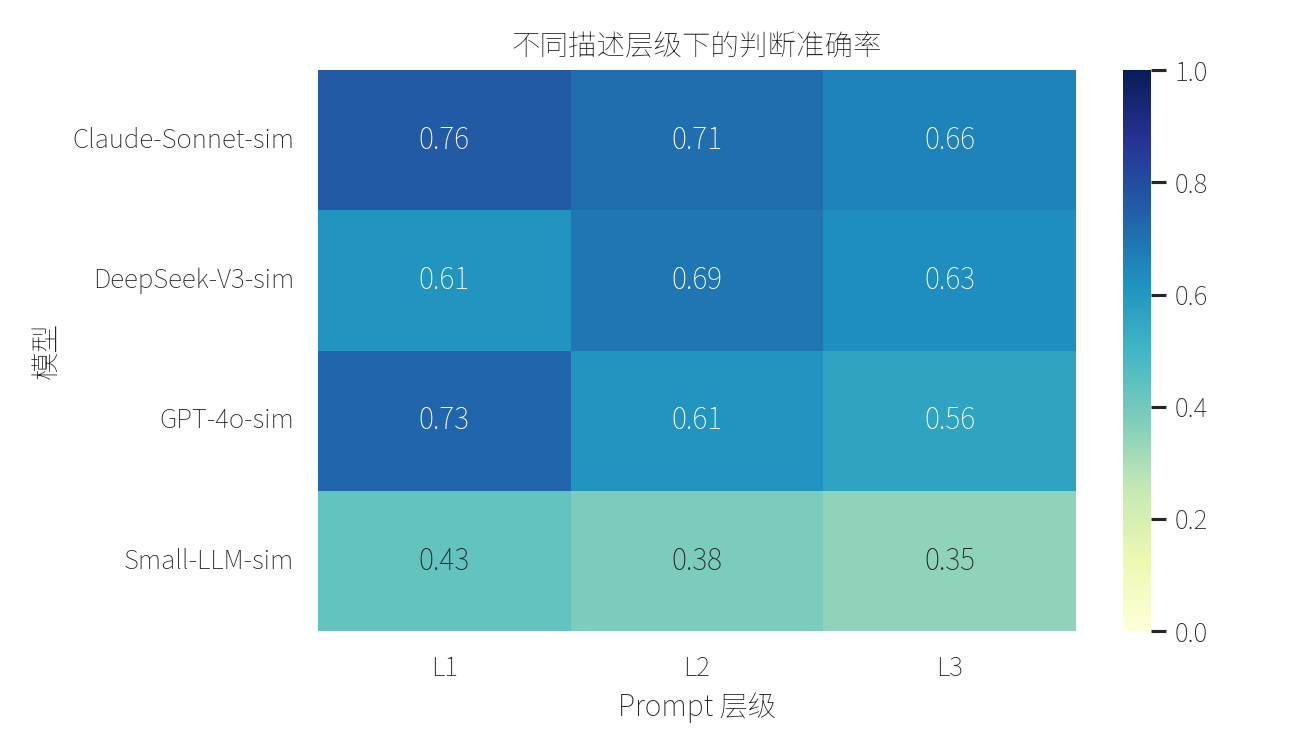
\includegraphics[width=0.82\textwidth]{accuracy_heatmap.png}
    \bicaption{不同模型在 Prompt 层级上的准确率热力图}{Accuracy heatmap across prompt levels}
    \label{fig:accuracy}
\end{figure}

\section{模型行为边界}

图 \ref{fig:radar} 可用于对比不同模型在准确率、一致性、公式使用、坐标建模和噪声敏感性等维度上的综合表现。正式写作时，应结合具体指标解释各模型的优势和边界。

\begin{figure}[htbp]
    \centering
    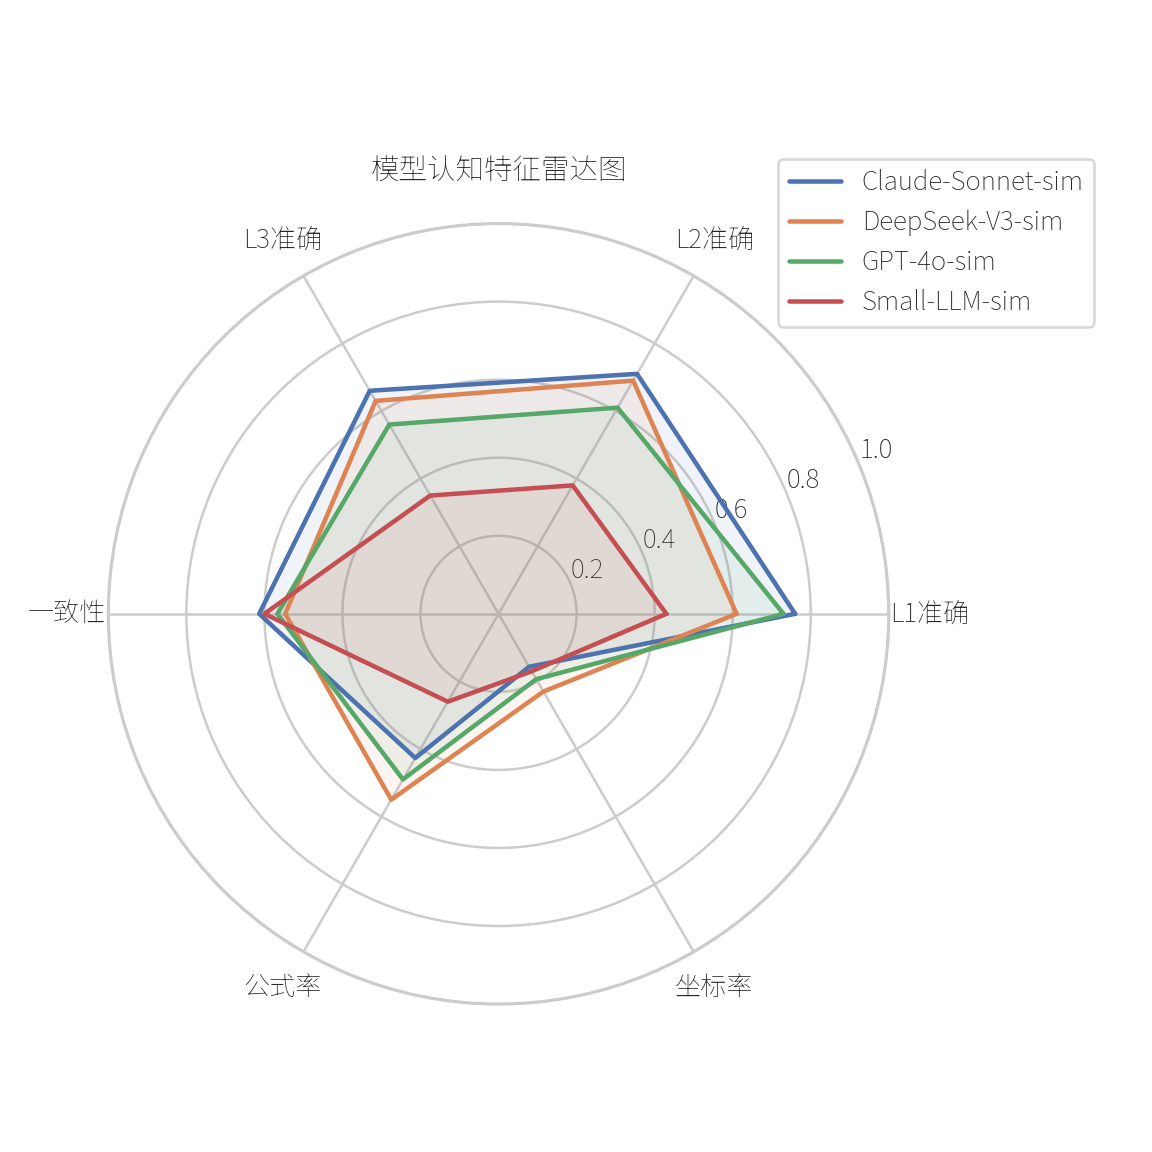
\includegraphics[width=0.78\textwidth]{model_radar.png}
    \bicaption{模型行为特征雷达图}{Radar chart of model behavioral features}
    \label{fig:radar}
\end{figure}

\section{无关噪声对判断的影响}

该部分可结合 \texttt{outputs/tables/noise\_flip\_rate.csv}，分析不同噪声条件是否引起模型判断翻转。重点关注 borderline 场景，因为临界场景更容易放大模型的不稳定性。

\section{失效模式分析}

可结合 \texttt{outputs/tables/failure\_modes.csv} 和错误样例，分析错误主要集中在哪些类别。建议至少选取 2 到 3 条典型回复，说明模型如何出现概念混淆、计算崩溃或噪声牵引。

\section{关联规则发现}

可从 \texttt{outputs/tables/outcome\_rules.csv} 中选取支持度、置信度和提升度较高的规则，解释“描述层级、干扰条件、临界性”如何共同诱发某类判断或错误模式。该部分是体现数据挖掘方法价值的重点。
      % 实验结果与分析框架
% ============================================================
% 4. 结尾部分
% ============================================================

% 结论
% !Mode:: "TeX:UTF-8"

\chapter{结\quad 论}

\section{全文总结}

本文构建了一个面向大语言模型空间推理行为的数据挖掘框架。项目通过多层级 Prompt、无关噪声扰动和可解释行为特征，能够从准确率、逻辑一致性、噪声敏感性和失效模式等角度分析模型能力边界。当前版本已经形成完整的代码流程和报告结构，后续可进一步补充真实模型多轮采样结果，并对关键发现进行统计检验。

\section{未来展望}

后续工作可以从三方面展开：第一，扩大模型和重复采样数量，提高结论稳定性；第二，引入更严格的几何基准或人工复核机制，提升参考标签可信度；第三，将该方法扩展到电梯通行、门洞转向、房间路径规划等更多空间任务，以验证模型空间建模能力的泛化边界。
    % 建议将“结论”独立于章节

% 参考文献
\cleardoublepage
%\nocite{*}
\bibliographystyle{plainnat}
\bibliography{references/reference}

% 项目成果（如需展示，可取消注释）
%% !Mode:: "TeX:UTF-8"

\chapter{项目分工与成果说明}

\begin{publist}
    \item Prompt 设计与实验矩阵：构建 L1/L2/L3 三层级 Prompt 和 5 类干扰条件。
    \item 数据采集：支持 mock、DF/OpenAI-compatible、OpenAI、Anthropic、DeepSeek 等 provider。
    \item 特征工程：抽取最终判断、推理步骤、公式使用、坐标建模和错误类型。
    \item 数据挖掘：完成准确率、层级一致性、噪声翻转率、聚类和 FP-Growth 关联规则分析。
    \item 可视化与报告：生成热力图、雷达图、聚类图、统计表和课程报告框架。
\end{publist}


% 致谢
% !Mode:: "TeX:UTF-8"

\chapter{致\quad 谢}

\defaultfont

感谢北京工业大学相关课程提供的数据挖掘实践机会。本项目的完成依赖于课程任务对问题定义、数据采集、特征抽取和挖掘分析的完整要求，也受益于开源 Python 生态中 Pandas、scikit-learn、mlxtend、Matplotlib 等工具的支持。

感谢小组成员在实验设计、API 采集、特征工程、模型分析、可视化和报告撰写中的分工协作。后续将继续完善真实模型实验数据和报告中的定量分析部分。


% 附录
% !Mode:: "TeX:UTF-8"

\chapter*{附\quad 录}
\addcontentsline{toc}{chapter}{附\quad 录}
\markboth{附\quad 录}{附\quad 录}

\section*{A. 项目运行命令}

\begin{lstlisting}[language=Python,caption={项目基础运行命令}]
python scripts/01_generate_prompts.py
python scripts/02_collect_responses.py --provider mock
python scripts/03_build_features.py
python scripts/04_analyze.py
\end{lstlisting}

若使用真实 API，应先在 shell 中设置环境变量，避免将密钥写入仓库文件。

\section*{B. 正式提交前待补充清单}

\begin{itemize}
    \item 修改封面中的学院、课程、指导教师和职称；
    \item 根据最终采集结果更新摘要中的样本量和结论；
    \item 在第 5 章补充关键表格数值和图表解释；
    \item 从原始回复中挑选典型错误样例；
    \item 检查参考文献是否与正文引用一致。
\end{itemize}


\end{document}
